\documentclass[
  ams,
  uplatex]{U-AizuGT}

\usepackage{pifont}
\usepackage{cite}
\usepackage[dvipdfmx]{graphicx}
\usepackage[dvipdfmx]{hyperref}

% ハイフネーション禁止
\hyphenpenalty=10000\relax
\exhyphenpenalty=10000\relax
\sloppy


% ここまで


\title{Writing a Thesis Using Markdown}
\author{Sachiko Tajima}
\studentid{s1250117}
\supervisor{Prof. Yutaka Watanobe}
\makeatletter
\@ifpackageloaded{subfig}{}{\usepackage{subfig}}
\@ifpackageloaded{caption}{}{\usepackage{caption}}
\captionsetup[subfloat]{margin=0.5em}
\AtBeginDocument{%
\renewcommand*\figurename{Figure}
\renewcommand*\tablename{Table}
}
\AtBeginDocument{%
\renewcommand*\listfigurename{List of Figures}
\renewcommand*\listtablename{List of Tables}
}
\@ifpackageloaded{float}{}{\usepackage{float}}
\floatstyle{ruled}
\@ifundefined{c@chapter}{\newfloat{codelisting}{h}{lop}}{\newfloat{codelisting}{h}{lop}[chapter]}
\floatname{codelisting}{Code}
\newcommand*\listoflistings{\listof{codelisting}{List of Listings}}
\makeatother

\bibliographystyle{ieicetr}






\begin{document}
    \maketitle
    
    \hypertarget{abstract}{%
    \section{Abstract}\label{abstract}}
    
    This is a template writtten is a Markdown following the University of
    Aizu graduation thesis format \cite{graduation-thesis}. If you have any
    quessstions or something you don't understand, just refer to
    kuee-thesis-markdown \cite{kuee-thesis-markdown} .
    
    \hypertarget{introduction}{%
    \section{Introduction}\label{introduction}}
    
    If you want to put figure or graph in thesis, write in the text as in
    \LaTeX writing.
    
    The \LaTeX Distribution kit includes the following files in table
    \ref{tab:kit} .
    
    \begin{table}[htbp]
      \caption{The kit distribution}\label{tab:kit}
      \begin{center}
        \begin{tabular}{ll}
          \verb+U-AizuGT.cls+ &  \LaTeX2e{} 's document classfile       \\
          \verb+ieicetr.bst+ & document style file \cite{ieicetr} \\
          \verb+thesis.bib+ & references file              \\
        \end{tabular}
      \end{center}
    \end{table}
    
    \hypertarget{reference}{%
    \subsection{Reference}\label{reference}}
    
    Nara suteki daigaku \cite{nara-nice} tekina.
    
    \hypertarget{table}{%
    \subsection{Table}\label{table}}
    
    aiueo kakikukeko sashisuseso tatituteto naninuneno hahihuheho mamimumemo
    yayuyo rarirurero wawon.
    
    \begin{table}[htbp]
      \caption{Sample of Figure $\cdot$ Table}\label{tab:fig}
      \begin{center}
        \begin{tabular}{|l|r|}
          \hline
          \verb+\textwidth+ & 424pt + 1cm  \\ \hline
          \verb+\textheight+ & 604pt + 67pt \\ \hline
          \verb+\oddsidemargin+ & 0pt          \\ \hline
          \verb+\evensidemargin+ & 0pt          \\ \hline
          \verb+\topmargin+ & 0pt          \\ \hline
          \verb+\headheight+ & 0pt          \\ \hline
          \verb+\headsep+ & 0pt          \\ \hline
          \verb+\footskip+ & 0pt          \\ \hline
        \end{tabular}
      \end{center}
    \end{table}
    
    \hypertarget{figure}{%
    \subsection{Figure}\label{figure}}
    
    \begin{figure}[htbp]
      \centering
      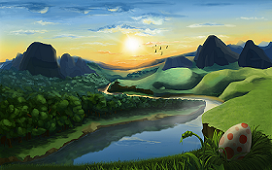
\includegraphics[scale = 1.0]{image.png}
      \caption{hogehoge}\label{fig:hogehoge}
    \end{figure}
    
    \hypertarget{material-methods}{%
    \section{Material \& Methods}\label{material-methods}}
    
    text tessssx ttexte
    
    \hypertarget{results}{%
    \section{Results}\label{results}}
    
    t e x t t e s s ss x t t exte
    
    \hypertarget{conclusion}{%
    \section{Conclusion}\label{conclusion}}
    
    text tes sssx tt exte
    
    \hypertarget{bobliography}{%
    \section{Bobliography}\label{bobliography}}
    
    text tess ssxt text e
    
    \hypertarget{acknowledgements}{%
    \section{Acknowledgements}\label{acknowledgements}}
    
    texttessssxttexte

        \bibliography{thesis.bib}
    

\end{document}
